\begin{frame}
  \begin{center}
    \LARGE <<Разработка тарифов>>
  \end{center}

  \begin{center}
      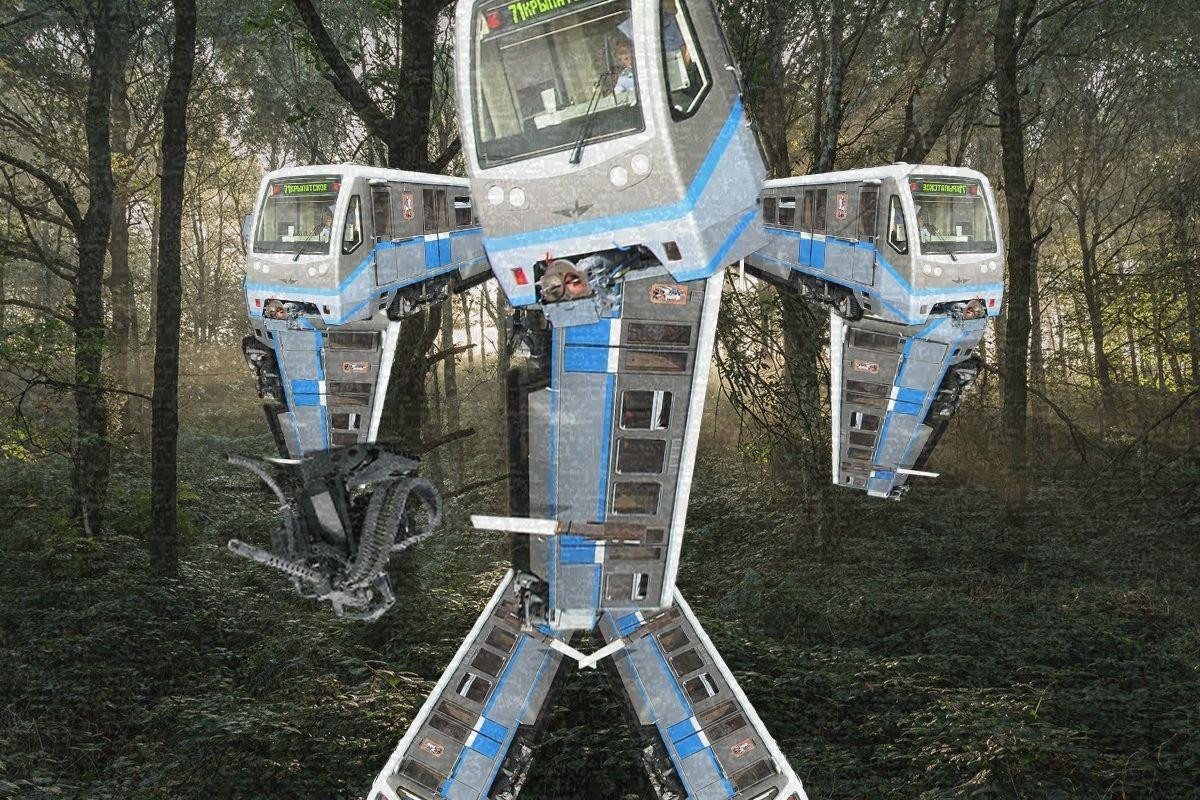
\includegraphics[width=5cm]{memes/d-meme.jpg}
  \end{center}

  \begin{itemize}
  \item Идея задачи --- Олег Мингалёв, Google
  \item Идея задачи --- Григорий Резников, МГУ
  \item Разработка задачи --- Константин Амеличев, ВШЭ
  \end{itemize}

\end{frame}

\begin{frame}{Постановка задачи}

  \begin{itemize}
  \item Дано дерево на $n$ вершинах и $m$ путей
  \item Требуется задать каждой вершине цвет $c_v$
  \item Вдоль пути цвета должны быть расположены монотонно
  \item Максимальное из чисел должно быть как можно меньше
  \end{itemize}

\end{frame}

\begin{frame}{Решение за $\O(n^n \cdot nm)$ (6 баллов)}
  \begin{itemize}
  \item Если раскраска существует, то она существует и с цветами от 1 до $n$
  \item Переберем все раскраски и проверим, что числа вдоль путей возрастают
  \end{itemize}
\end{frame}
\begin{frame}{Решение за $\O(2^n \cdot nm)$ (16 баллов)}
  \begin{itemize}
  \item Разделим ребра на покрытые и не покрытые путями
  \item Ребра второго типа разбивают задачу на несколько меньших задач
  \item Ребра первого типа задают сравнение --- либо $c_v < c_u$, либо $c_u < c_v$
  \end{itemize}
\end{frame}
\begin{frame}{Решение за $\O(2^n \cdot nm)$ (16 баллов)}
  \begin{itemize}
  \item Переберем все возможные сравнения
  \item Рассмотрим вершины в порядке топологической сортировки
  \item Задаем вершине минимальный доступный цвет
  \item Проверяем, что раскраска корректна
  \end{itemize}
\end{frame}

\begin{frame}{Граф --- звезда (+8 баллов)}
  \begin{itemize}
  \item Длина каждого пути не больше 3
  \item Построим граф на путях
  \item Проведем между пересекающимися путями рёбра вида ``эти пути ориентированы одинаково'' или ``эти
    пути ориентированы по-разному''.
  \end{itemize}
\end{frame}

\begin{frame}{Граф --- звезда (+8 баллов)}
  \begin{itemize}
  \item Выбор направления одного пути задает направления во всей компоненте.
  \item Возможно, ответа вообще нет (есть само-противоречащий цикл)
  \item Если же ориентировать пути удалось, то в оптимальной раскраске цвета не больше 3.
  \end{itemize}
\end{frame}

\begin{frame}{Пути не пересекаются, $\O(n \log^2 n)$ (+10 баллов)}
  \begin{itemize}
    \item Раскраска точно существует
    \item Сделаем бинарный поиск по максимальному цвету
    \item Проверим, возможно ли раскрасить дерево в $k$ цветов
  \end{itemize}
\end{frame}

\begin{frame}{Пути не пересекаются, $\O(n \log^2 n)$ (+10 баллов)}
  \begin{itemize}
    \vspace{-1em}
  \item Динамика по поддеревьям.
  \item Для определённости считаем, что ребро $v \rightarrow parent_v$ направлено так, что $c_v < c_{parent_v}$.
  \item Тогда лучше красить $v$ в минимально возможный цвет, т.к. покраска $c_v = k$ задаёт ограничения на родителя:
    $c_{parent_v} \ge k + 1$.
  \item Скажем, что $dp[v]$ --- минимальный возможный цвет $v$, согласованный с поддеревом.
    В силу симметрии, максимально возможный цвет (имеет смысл если $c_v > c_{parent_v}$) равен $k + 1 - dp[v]$
  \end{itemize}
\end{frame}

\begin{frame}{Пути не пересекаются, $\O(n \log^2 n)$ (+10 баллов)}
  \begin{itemize}
    \item Для вершины $v$ есть набор ограничений
    \item Если через $v$ ввысь идёт вертикальный путь из поддерева $u$, то $dp[v] \ge dp[u] + 1$
    \item Если через $v$ проходит путь из поддерева $a$ в поддерево $b$, то:
    \begin{enumerate}
        \item $dp[v] \ge dp[a] + 1$
        \item $dp[v] \le k - dp[b]$
    \end{enumerate}
    \item Но мы не знаем, в какую сторону направлен путь, кто же $a$, а кто же $b$?
  \end{itemize}
\end{frame}

\begin{frame}{Пути не пересекаются, $\O(n \log^2 n)$ (+10 баллов)}
  \begin{itemize}
    \item Попробуем и так, и так
    \item $dp[v] \in [dp[a] + 1, k - dp[b]]$ или $dp[v] \in [dp[b] + 1, k - dp[a]]$
    \item Хотим решить систему таких условий. Для каждого пути выпишем два отрезка и сделаем сканлайн.
    \item Найдем самую левую точку, покрытую отрезками всех цветов.
    \item Решение за $\O(n \log^2 n)$.
  \end{itemize}
\end{frame}

\begin{frame}{Пути не пересекаются, $\O(n \log n)$ (+16~баллов)}
  \begin{itemize}
    \item Заметим, что мы взяли ограничения в два множества --- $L$ и $R$
    \item $max(L) + 1 \le min(k - R) \iff max(L) + max(R) \le k - 1$
    \item $dp[v] = max(L) + 1$
    \item Надо разложить пары $dp[a_i],\,dp[b_i]$ по двум множествам
    \item При этом $L$ уже содержит какие-то ограничения
  \end{itemize}
\end{frame}

\begin{frame}{Пути не пересекаются, $\O(n \log n)$ (+16~баллов)}
  \begin{itemize}
    \item Зафиксируем, что будет больше --- $max(L)$ или $max(R)$
    \item Тогда в каждой паре разложение определится однозначно --- логично отправить максимум в то множество, где максимум больше.
    \item Проверим оба варианта на условие $max(L) + max(R) \le k - 1$ и возьмём наилучший.
  \end{itemize}
\end{frame}

\begin{frame}{Полное решение (100 баллов)}
  \begin{itemize}
    \item Как в графе-звёздочке, строим новый граф.
    \item Для каждого ребра становится известен класс эквивалентности.
    \item Внутри классов эквивалентности мы знаем ориентацию ребер, относительно <<основного>> ребра внутри класса.
  \end{itemize}
\end{frame}

\begin{frame}{Полное решение (100 баллов)}
  \begin{itemize}
  \item Бинарный поиск по ответу, такая же $dp[v]$.
  \item Рёбра в том же классе эквивалентности задают конкретные $L/R$ ограничения.
  \item Все остальные классы характеризуются множествами ограничений $A, B$ (и нужно одно отправить в $L$, другое в $R$).
  \item Внутри этих множеств достаточно взять $a,\,b$ так, что $dp[a] \ge dp[a'],\ dp[b] \ge dp[b']$.
  \item Дальше решаем так же, как в прошлый раз. В зависимости от подсчета динамики решили за $\O(n \log^2 n)$ или $\O(n \log n)$
  \end{itemize}
\end{frame}
